\documentclass[conference]{IEEEtran}

\usepackage[utf8]{inputenc}
\usepackage[T1]{fontenc}
\usepackage{cite}
\usepackage{amsmath,amssymb}
\usepackage{booktabs}
\usepackage{array}
\usepackage{graphicx}
\usepackage{xcolor}
\usepackage{tikz}
\usetikzlibrary{arrows.meta,positioning,fit,shapes.geometric}
\usepackage{url}
\usepackage[hidelinks]{hyperref}

\newcommand{\etal}{\textit{et al.}}
\newcommand{\pipeline}{Source--Bronze--Silver--Gold}

\begin{document}

\title{Quasi-Experimental Evaluation of a Hash-linked Tamper-evident Ledger for Data Pipeline Integrity Verification}

\author{\IEEEauthorblockN{Nguyen Ngoc Son}
\IEEEauthorblockA{Faculty of Cyber Security\\
KMA, Vietnam\\
Email: sonnn.tech@gmail.com}}

\maketitle

\begin{abstract}
Các hệ thống Data Pipeline hiện đại xử lý dữ liệu qua nhiều giai đoạn như thu thập, chuyển đổi, lưu trữ và phục vụ phân tích. Tuy nhiên, sau khi pipeline hoàn tất, nhiều nền tảng chưa có cơ chế độc lập để kiểm chứng rằng dữ liệu đã lưu vẫn khớp với trạng thái được sinh ra tại thời điểm thực thi. Nhật ký kiểm toán, checksum ở tầng ứng dụng và dashboard giám sát đều hữu ích, nhưng thường nằm trong cùng ranh giới tin cậy với dữ liệu hoặc chỉ phản ánh trạng thái khi pipeline đang chạy. Bài báo này trình bày một nghiên cứu đánh giá bán thực nghiệm đối với cơ chế \hashledger{} nhằm kiểm chứng tính toàn vẹn dữ liệu trong Data Pipeline. Cơ chế đề xuất ghi nhận bằng chứng ở từng stage, bao gồm số lượng bản ghi, schema hash, batch hash, block hash, liên kết previous hash và sự kiện lineage. Verification engine tính toán lại các bằng chứng sau xử lý và trả về trạng thái vi phạm toàn vẹn nếu có sai lệch. Nghiên cứu so sánh điều kiện sạch và điều kiện bị can thiệp, đánh giá khả năng truy vết đến first broken block và lineage event liên quan, đồng thời ước lượng overhead theo các mức record count khác nhau. Kết quả thực nghiệm trên nguyên mẫu Databricks cho thấy tất cả tamper scenarios được định nghĩa trước đều được phát hiện trong phạm vi kiểm thử, trong khi điều kiện sạch không tạo false positive trong dashboard export quan sát được. Overhead tăng theo record count, nhưng kết quả vẫn bị giới hạn bởi biến thiên môi trường cloud compute và số lần lặp benchmark còn hạn chế. Đóng góp của bài báo không phải là một hệ thống Blockchain đầy đủ, mà là đánh giá có kiểm soát một cơ chế hash-linked tamper-evident phục vụ bảo đảm tính toàn vẹn dữ liệu trong Data Pipeline.
\end{abstract}

\begin{IEEEkeywords}
Tính toàn vẹn dữ liệu, tamper-evident ledger, hash chain, data pipeline, bán thực nghiệm, an toàn thông tin, data lineage.
\end{IEEEkeywords}

\section{Introduction}

Data pipelines have become critical components of analytical and operational information systems. A typical pipeline receives source data, transforms it through intermediate layers, persists curated outputs, and exposes them to reporting or downstream applications. In many lakehouse and warehouse architectures, this lifecycle is represented by stages such as \pipeline. While these stages improve data organization and observability, they do not automatically guarantee that data remains unchanged after the pipeline has finished.

This problem is a cybersecurity and information assurance concern. If a privileged user, compromised credential, or insider modifies data after execution, the pipeline may still appear successful in the orchestration tool. Conventional monitoring can confirm that a job ran, but it may not independently verify whether the stored data has been altered later. Audit logs and database logs can help, but they usually remain inside the same administrative trust boundary as the protected data. Application-level checksums can detect simple mismatches, yet they are often not chained across pipeline stages and may not provide a clear trace to the affected transformation.

This paper investigates a lightweight alternative: a hash-linked tamper-evident ledger. A tamper-evident mechanism does not prevent modification. Instead, it provides evidence that a modification has occurred. A hash-linked ledger stores evidence records in sequence, where each block includes a hash of the previous block. If a block payload or prior link is changed, later verification can detect that the chain no longer matches.

\subsection{Research Gap}

Several existing mechanisms address parts of the data integrity problem. Database audit logs record operations, but administrators with sufficient privileges may alter both data and logs. Application-level checksums can validate a dataset snapshot, but they are commonly isolated and do not preserve stage-to-stage linkage. Full decentralized blockchains provide stronger immutability properties through consensus and replicated nodes, but their operational overhead and architectural complexity are often unnecessary for an internal data pipeline integrity experiment. Pipeline monitoring observes execution status, but it does not necessarily provide post-execution integrity evidence.

The gap addressed in this paper is the lack of a controlled evaluation of a lightweight hash-linked ledger for multi-stage data pipeline integrity verification. The study focuses on whether such a mechanism can detect predefined tamper scenarios, identify the first broken block and related lineage context, and quantify the additional runtime overhead under a constrained experimental environment.

\subsection{Research Questions}

The study is guided by four research questions:

\begin{itemize}
    \item \textbf{RQ1:} Can a hash-linked ledger and verification engine detect unauthorized changes to pipeline data, ledger payloads, and chain links?
    \item \textbf{RQ2:} Can the mechanism identify the first broken block, affected stage, and related lineage event?
    \item \textbf{RQ3:} What additional runtime overhead does the mechanism introduce as record count changes?
    \item \textbf{RQ4:} Which uncontrolled variables in the experimental environment limit the strength of the conclusions?
\end{itemize}

\subsection{Contributions}

This work makes three contributions. First, it defines a bounded tamper-evident mechanism for data pipeline integrity verification using stage-level batch hashes, block hashes, previous-hash links, and lineage events. Second, it designs a quasi-experimental evaluation with clean, tampered, and benchmark conditions. Third, it reports empirical observations and validity limitations instead of claiming general blockchain-level immutability or strong causal proof.

\section{Methodology}

\subsection{Justification for Quasi-Experimental Design}

This study follows a quasi-experimental methodology because the intervention can be implemented and measured, but the environment cannot be fully controlled. A true experiment would require random assignment, controlled compute resources, stable network conditions, repeated execution under identical resource states, and a representative population of real attackers. These assumptions are not realistic in the selected Databricks-based environment.

The experiment controls what can be controlled: the pipeline structure, synthetic data generation seed, predefined tamper scenarios, verification logic, measured variables, and run procedure. The experiment documents what cannot be controlled: cloud scheduling, warm-up behavior, cache state, network latency, and the fact that tamper scenarios are researcher-defined proxies rather than a random sample of real-world attacks. Therefore, the study reports quasi-experimental evidence of association between the treatment and observed integrity outcomes, not a universal causal claim.

\subsection{Treatment and Control Conditions}

The treatment is the addition of a hash-linked tamper-evident ledger, lineage recorder, and verification engine to a standard data pipeline. The control condition depends on the research question. For detection and traceability, the clean pipeline state with no tamper scenario acts as the pre-test control. For overhead measurement, the baseline pipeline without ledger and verification instrumentation acts as the non-equivalent control.

\begin{figure}[t]
\centering
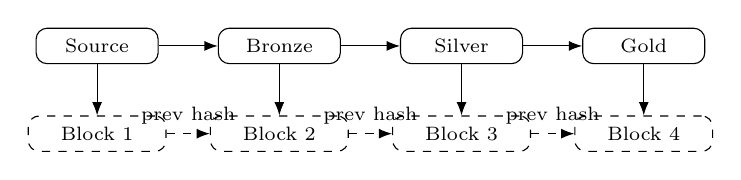
\begin{tikzpicture}[node distance=0.75cm,>=Latex, every node/.style={font=\scriptsize}]
\tikzstyle{stage}=[draw, rounded corners, minimum width=1.55cm, minimum height=0.45cm, align=center]
\tikzstyle{ledger}=[draw, dashed, rounded corners, minimum width=1.75cm, minimum height=0.45cm, align=center]
\node[stage] (src) {Source};
\node[stage, right=of src] (brz) {Bronze};
\node[stage, right=of brz] (slv) {Silver};
\node[stage, right=of slv] (gld) {Gold};
\node[ledger, below=0.65cm of src] (b1) {Block 1};
\node[ledger, below=0.65cm of brz] (b2) {Block 2};
\node[ledger, below=0.65cm of slv] (b3) {Block 3};
\node[ledger, below=0.65cm of gld] (b4) {Block 4};
\draw[->] (src) -- (brz);
\draw[->] (brz) -- (slv);
\draw[->] (slv) -- (gld);
\draw[->] (src) -- (b1);
\draw[->] (brz) -- (b2);
\draw[->] (slv) -- (b3);
\draw[->] (gld) -- (b4);
\draw[->, dashed] (b1) -- node[above]{prev hash} (b2);
\draw[->, dashed] (b2) -- node[above]{prev hash} (b3);
\draw[->, dashed] (b3) -- node[above]{prev hash} (b4);
\end{tikzpicture}
\caption{Hash-linked tamper-evident ledger for a multi-stage data pipeline.}
\label{fig:architecture}
\end{figure}

\subsection{Hypotheses}

\begin{table}[t]
\caption{Research Hypotheses}
\centering
\begin{tabular}{p{0.12\linewidth}p{0.75\linewidth}}
\toprule
\textbf{ID} & \textbf{Hypothesis} \\
\midrule
H1 & The treatment detects all predefined tamper scenarios, while the clean condition remains valid. \\
H2 & The treatment identifies the first broken block and links it to a corresponding lineage event. \\
H3 & The treatment increases runtime compared with the baseline pipeline, and overhead changes with record count. \\
H4 & Uncontrolled variables prevent strong true-experimental causal claims. \\
\bottomrule
\end{tabular}
\label{tab:hypotheses}
\end{table}

\subsection{Variables}

The independent variables include tamper scenario, record count, pipeline stage, security mechanism, and run condition. The dependent variables include verification outcome, detection rate, first-broken-block accuracy, traceability completeness, security overhead, baseline duration, secured duration, and verification duration.

\begin{table}[t]
\caption{Core Experimental Variables}
\centering
\begin{tabular}{p{0.20\linewidth}p{0.26\linewidth}p{0.38\linewidth}}
\toprule
\textbf{Variable} & \textbf{Type} & \textbf{Purpose} \\
\midrule
Tamper scenario & Categorical IV & Stimulus for detection and traceability. \\
Record count & Ordinal IV & Scaling factor for overhead. \\
Pipeline stage & Categorical IV & Context for block and lineage mapping. \\
Security mechanism & Binary IV & Control versus treatment comparison. \\
Verification outcome & Categorical DV & Main detection result. \\
Detection rate & Numeric DV & Ratio of detected tamper scenarios. \\
Security overhead & Numeric DV & Additional runtime cost of treatment. \\
\bottomrule
\end{tabular}
\label{tab:variables}
\end{table}

\section{Thiết kế và môi trường thực nghiệm}

\subsection{Nguyên mẫu Data Pipeline}

Nguyên mẫu triển khai một pipeline phân tích gồm bốn stage: Source, Bronze, Silver và Gold. Dữ liệu nguồn được sinh tổng hợp bằng random seed cố định nhằm hỗ trợ khả năng tái lập. Bronze lưu dữ liệu sau khi ingest, Silver thực hiện chuẩn hóa và transformation, còn Gold lưu kết quả tổng hợp phục vụ phân tích. Mỗi stage sinh ra bằng chứng integrity và ghi vào ledger.

Đối với mỗi stage, ledger ghi nhận stage name, record count, schema hash, batch hash, block hash, previous block hash, transformation metadata, timestamp và pipeline run identifier. Batch hash đại diện cho nội dung đã canonicalize của output tại stage. Schema hash đại diện cho cấu trúc dữ liệu. Block hash là digest mật mã của payload trong block. Previous hash liên kết block hiện tại với block trước đó trong cùng pipeline run.

\subsection{Cấu trúc block ledger}

Cấu trúc block được thiết kế để đủ đơn giản cho MVP nhưng vẫn bảo toàn các bằng chứng chính cần cho verification. Mỗi block chứa ba nhóm thông tin: định danh run, evidence của stage và chain metadata. Định danh run giúp gom các block thuộc cùng một lần chạy pipeline. Evidence của stage giúp phát hiện thay đổi dữ liệu hoặc schema. Chain metadata giúp phát hiện việc sửa payload hoặc phá liên kết block.

\begin{table}[t]
\caption{Cấu trúc logic của một ledger block}
\centering
\begin{tabular}{p{0.30\linewidth}p{0.54\linewidth}}
\toprule
\textbf{Trường} & \textbf{Ý nghĩa} \\
\midrule
pipeline\_run\_id & Định danh một lần chạy pipeline. \\
stage & Source, Bronze, Silver hoặc Gold. \\
record\_count & Số lượng bản ghi tại stage. \\
schema\_hash & Hash của cấu trúc schema. \\
batch\_hash & Hash của nội dung dữ liệu canonicalized. \\
previous\_hash & Block hash của block trước đó. \\
block\_hash & Hash của payload block hiện tại. \\
transformation & Metadata mô tả transformation. \\
\bottomrule
\end{tabular}
\label{tab:block_structure}
\end{table}

\begin{figure}[t]
\centering
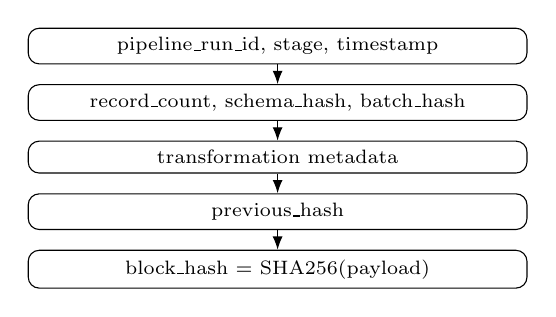
\begin{tikzpicture}[node distance=0.25cm,>=Latex, every node/.style={font=\scriptsize}]
\tikzstyle{field}=[draw, rounded corners, text width=6.1cm, align=center, minimum height=0.35cm]
\node[field] (f1) {pipeline\_run\_id, stage, timestamp};
\node[field, below=of f1] (f2) {record\_count, schema\_hash, batch\_hash};
\node[field, below=of f2] (f3) {transformation metadata};
\node[field, below=of f3] (f4) {previous\_hash};
\node[field, below=of f4] (f5) {block\_hash = SHA256(payload)};
\draw[->] (f1) -- (f2);
\draw[->] (f2) -- (f3);
\draw[->] (f3) -- (f4);
\draw[->] (f4) -- (f5);
\end{tikzpicture}
\caption{Block payload và hash evidence trong ledger.}
\label{fig:block_structure}
\end{figure}

Verification engine tính toán lại bằng chứng ở từng stage và so sánh với ledger đã lưu. Sai lệch content hash chỉ ra khả năng data tampering. Sai lệch record count chỉ ra khả năng insert hoặc delete. Sai lệch block payload chỉ ra ledger tampering. Sai lệch previous hash chỉ ra chain link bị phá vỡ.

\subsection{Thuật toán tạo ledger và kiểm chứng}

Bảng~\ref{tab:algo_ledger} mô tả thuật toán tạo ledger ở mức khái niệm. Tại mỗi stage, pipeline canonicalize dữ liệu, tính schema hash, batch hash, lấy previous hash của block trước, sau đó tạo block hash cho payload hiện tại.

\begin{table}[t]
\caption{Algorithm 1: Ledger Generation}
\centering
\begin{tabular}{p{0.08\linewidth}p{0.76\linewidth}}
\toprule
1 & Nhận output dataset của stage hiện tại. \\
2 & Chuẩn hóa thứ tự cột và bản ghi để canonicalize dữ liệu. \\
3 & Tính schema\_hash và batch\_hash bằng SHA-256. \\
4 & Lấy previous\_hash từ block trước trong cùng pipeline\_run\_id. \\
5 & Tạo block payload gồm run id, stage, counts, hashes và metadata. \\
6 & Tính block\_hash = SHA256(block payload). \\
7 & Ghi block vào blockchain\_ledger và ghi lineage event. \\
\bottomrule
\end{tabular}
\label{tab:algo_ledger}
\end{table}

Bảng~\ref{tab:algo_verify} mô tả thuật toán verification. Điểm quan trọng là verification không chỉ so sánh dữ liệu với batch hash, mà còn kiểm tra block hash và previous hash để phát hiện sai lệch trong ledger hoặc chain link.

\begin{table}[t]
\caption{Algorithm 2: Integrity Verification}
\centering
\begin{tabular}{p{0.08\linewidth}p{0.76\linewidth}}
\toprule
1 & Đọc toàn bộ blocks theo pipeline\_run\_id và thứ tự stage. \\
2 & Với mỗi block, tính lại record count, schema hash và batch hash. \\
3 & Nếu record count khác ledger, trả về RECORD\_COUNT\_MISMATCH. \\
4 & Nếu batch hash khác ledger, trả về DATA\_TAMPERED. \\
5 & Tính lại block hash từ payload đã lưu. \\
6 & Nếu block hash không khớp, trả về BLOCK\_TAMPERED. \\
7 & Nếu previous hash không khớp block trước, trả về CHAIN\_BROKEN. \\
8 & Nếu không có sai lệch, trả về VALID. \\
\bottomrule
\end{tabular}
\label{tab:algo_verify}
\end{table}

\subsection{Tamper Scenarios}

Nghiên cứu đánh giá sáu tamper scenarios và một clean scenario. Clean scenario, ký hiệu NONE, được dùng để quan sát false positive. Các tamper scenarios bao gồm sửa giá trị giao dịch, xóa bản ghi, chèn bản ghi giả, sửa batch hash đã lưu, sửa transformation metadata và sửa previous-hash link.

\begin{table}[t]
\caption{Tamper scenarios và outcome kỳ vọng}
\centering
\begin{tabular}{p{0.45\linewidth}p{0.39\linewidth}}
\toprule
\textbf{Scenario} & \textbf{Verification outcome kỳ vọng} \\
\midrule
NONE & VALID \\
MODIFY\_TRANSACTION\_AMOUNT & DATA\_TAMPERED \\
DELETE\_TRANSACTION & RECORD\_COUNT\_MISMATCH \\
INSERT\_FAKE\_TRANSACTION & RECORD\_COUNT\_MISMATCH \\
MODIFY\_LEDGER\_BATCH\_HASH & DATA\_TAMPERED \\
MODIFY\_LEDGER\_TRANSFORMATION & BLOCK\_TAMPERED \\
MODIFY\_LEDGER\_PREVIOUS\_HASH & CHAIN\_BROKEN \\
\bottomrule
\end{tabular}
\label{tab:scenarios}
\end{table}

\subsection{Môi trường và dữ liệu}

Thực nghiệm sử dụng Databricks Free Edition với PySpark và Delta Table. Dataset là dữ liệu giao dịch synthetic, không chứa dữ liệu cá nhân thật. Cấu hình mặc định dùng record count 10.000 và random seed 42. Benchmark dùng bốn mức record count: 1K, 5K, 10K và 50K. Việc dùng synthetic data giúp giảm rủi ro đạo đức và hỗ trợ tái lập, nhưng làm giảm external validity so với dữ liệu production.

\begin{table}[t]
\caption{Môi trường thực nghiệm}
\centering
\begin{tabular}{p{0.32\linewidth}p{0.52\linewidth}}
\toprule
\textbf{Thành phần} & \textbf{Giá trị} \\
\midrule
Compute & Databricks Free Edition / cloud workspace \\
Processing & PySpark, Delta Table \\
Hash function & SHA-256 \\
Dataset & Synthetic transactions \\
Default size & 10.000 records \\
Benchmark sizes & 1K, 5K, 10K, 50K records \\
Seed & 42 \\
\bottomrule
\end{tabular}
\label{tab:environment}
\end{table}

\subsection{Quy trình thực nghiệm}

Quy trình thực nghiệm được mô tả trong Hình~\ref{fig:procedure}. Đầu tiên, môi trường và các Delta tables được khởi tạo. Tiếp theo, dữ liệu synthetic được sinh bằng seed cố định. Sau đó, pipeline baseline và pipeline có treatment được thực thi. Verification engine kiểm tra clean run. Một tamper scenario được áp dụng, rồi verification được chạy lại để đo detection và traceability. Trạng thái baseline được reset trước khi chuyển sang scenario tiếp theo. Cuối cùng, benchmark được chạy theo nhiều mức record count.

\begin{figure}[t]
\centering
\begin{tikzpicture}[node distance=0.32cm,>=Latex, every node/.style={font=\scriptsize}]
\tikzstyle{step}=[draw, rounded corners, text width=6.1cm, align=center, minimum height=0.41cm]
\node[step] (s1) {Khởi tạo môi trường và bảng};
\node[step, below=of s1] (s2) {Sinh dữ liệu synthetic};
\node[step, below=of s2] (s3) {Chạy baseline và treatment pipeline};
\node[step, below=of s3] (s4) {Verify điều kiện sạch};
\node[step, below=of s4] (s5) {Tiêm một tamper scenario};
\node[step, below=of s5] (s6) {Verify detection và traceability};
\node[step, below=of s6] (s7) {Reset baseline và lặp lại};
\node[step, below=of s7] (s8) {Benchmark theo record count};
\draw[->] (s1) -- (s2);
\draw[->] (s2) -- (s3);
\draw[->] (s3) -- (s4);
\draw[->] (s4) -- (s5);
\draw[->] (s5) -- (s6);
\draw[->] (s6) -- (s7);
\draw[->] (s7) -- (s8);
\end{tikzpicture}
\caption{Quy trình thực nghiệm cho clean run, tamper run và benchmark run.}
\label{fig:procedure}
\end{figure}

Các warm-up runs được đánh dấu và loại khỏi phần tổng hợp benchmark chính. Median overhead được ưu tiên hơn mean vì trạng thái cloud compute và cold start có thể tạo outlier. Benchmark sử dụng các mức record count 1K, 5K, 10K và 50K.

\section{Experimental Evaluation}

\subsection{Detection Results}

The clean condition produced VALID verification outcomes in the dashboard export used as evidence for the non-tampered state. The tamper experiments produced non-VALID outcomes for all predefined tamper scenarios. Table~\ref{tab:results} summarizes the observed outcomes. The result supports H1 within the bounded set of evaluated scenarios.

\begin{table}[t]
\caption{Observed Verification Results}
\centering
\begin{tabular}{p{0.42\linewidth}p{0.31\linewidth}p{0.12\linewidth}}
\toprule
\textbf{Scenario} & \textbf{Observed Outcome} & \textbf{Class} \\
\midrule
NONE & VALID & TN \\
MODIFY\_TRANSACTION\_AMOUNT & DATA\_TAMPERED & TP \\
DELETE\_TRANSACTION & RECORD\_COUNT\_MISMATCH & TP \\
INSERT\_FAKE\_TRANSACTION & RECORD\_COUNT\_MISMATCH & TP \\
MODIFY\_LEDGER\_BATCH\_HASH & DATA\_TAMPERED & TP \\
MODIFY\_LEDGER\_TRANSFORMATION & BLOCK\_TAMPERED & TP \\
MODIFY\_LEDGER\_PREVIOUS\_HASH & CHAIN\_BROKEN & TP \\
\bottomrule
\end{tabular}
\label{tab:results}
\end{table}

The observed detection rate is calculated as:

\begin{equation}
Detection\ Rate = \frac{TP}{TP + FN} \times 100\%.
\end{equation}

With six true positives and no observed false negative in the tampered scenarios, the detection rate is 100\% within the predefined test set. This result must not be interpreted as universal attack coverage. It only means that the mechanism detected the six tamper vectors selected for this experiment.

\subsection{Traceability Results}

The verification engine reports a first broken block when a mismatch is found. This block can be joined with lineage events using the pipeline run identifier. The sample lineage flow records Source-to-Bronze, Bronze-to-Silver, and Silver-to-Gold transformations, including input record count, output record count, transformation context, and status. For the evaluated tamper scenarios, the recorded first broken block and lineage context matched the affected stage at a coarse stage level. This supports H2, with the limitation that some stage values were recorded as approximate in the source report and should be verified by direct SQL export for a stronger claim.

\subsection{Overhead Results}

Security overhead is computed as:

\begin{equation}
Overhead = \frac{SecuredDuration - BaselineDuration}{BaselineDuration} \times 100\%.
\end{equation}

The approximate dashboard values show overhead increasing from about 160\% at 1K records to about 220\% at 50K records. Table~\ref{tab:overhead} summarizes the observed trend. The 5K case is close to the 1K case, which suggests the influence of cloud runtime variance. Overall, the evidence supports H3 with caveats.

\begin{table}[t]
\caption{Approximate Runtime Overhead by Record Count}
\centering
\begin{tabular}{p{0.30\linewidth}p{0.33\linewidth}p{0.22\linewidth}}
\toprule
\textbf{Record Count} & \textbf{Approx. Overhead} & \textbf{Evidence Type} \\
\midrule
1K & $\sim$160\% & Dashboard \\
5K & $\sim$155--160\% & Dashboard \\
10K & $\sim$180\% & Dashboard \\
50K & $\sim$220\% & Dashboard \\
\bottomrule
\end{tabular}
\label{tab:overhead}
\end{table}

Verification latency ranged from approximately 24 seconds to 31 seconds in recent runs, with one higher outlier. This observation is consistent with the quasi-experimental assumption that cold start and cloud compute scheduling cannot be fully controlled.

\subsection{Discussion}

The experimental evidence indicates that a hash-linked ledger can make post-execution tampering visible in a multi-stage pipeline. The mechanism is especially useful when the objective is not to prevent privileged writes directly, but to make unauthorized modification detectable during later verification. This aligns with tamper-evident design rather than tamper-proof design.

The result also clarifies the role of the word blockchain. The prototype uses a blockchain-inspired hash chain, but it does not implement distributed consensus, replicated nodes, mining, proof-of-work, proof-of-stake, or smart contracts. Therefore, the more precise term is hash-linked tamper-evident ledger. This distinction is important for construct validity and prevents overclaiming.

\section{Threats to Validity}

\subsection{Internal Validity}

The main internal validity threat is uncontrolled compute state. The experiment runs in a cloud-managed Databricks environment where cluster warm-up, cache state, scheduling, and resource allocation are not fully controlled. These factors can affect runtime overhead independently of the treatment. To reduce this threat, warm-up runs are excluded and median summaries are preferred.

Another internal threat is history effect. If tables are not reset correctly between tamper scenarios, stale data or stale ledger records may create false positives or false negatives. The procedure therefore includes an explicit RESET\_BASELINE step before moving to the next scenario.

\subsection{External Validity}

The experiment uses one Databricks workspace and synthetic transaction data. The results may not generalize to AWS Glue, on-premise Spark, dbt, Snowflake, or production lakehouse environments. Synthetic data also lacks the distribution skew, schema drift, missing values, and operational complexity of real production datasets. Future replication should use multiple environments and anonymized production-like data.

\subsection{Construct Validity}

The system should not be interpreted as a full blockchain. The evaluated construct is a hash-linked tamper-evident ledger. It provides integrity evidence through hashes and previous-hash links, but it does not provide decentralized consensus or public-chain immutability. Another construct threat is the detection-rate metric. The reported 100\% detection rate applies only to the six tamper scenarios selected for the experiment.

\subsection{Conclusion Validity}

The number of tamper scenarios, record-count levels, and benchmark repetitions is limited. This makes the results useful as quasi-experimental evidence but insufficient for strong statistical conclusions. The overhead values are approximate because they were taken from dashboard observations rather than a full exported raw benchmark dataset. At least thirty repeated runs per record-count level would be needed for confidence intervals, distribution plots, and stronger effect-size analysis.

\section{Kết luận và hướng phát triển}

Bài báo đã trình bày một đánh giá bán thực nghiệm đối với cơ chế Hash-linked Tamper-evident Ledger nhằm kiểm chứng tính toàn vẹn dữ liệu trong hệ thống Data Pipeline. Cơ chế này ghi nhận bằng chứng integrity ở từng stage và liên kết các ledger blocks thông qua previous hash. Verification engine tính toán lại record count, schema hash, batch hash, block hash và chain link để phát hiện modification sau xử lý.

Các quan sát thực nghiệm hỗ trợ các giả thuyết chính trong phạm vi bounded scope. Tất cả tamper scenarios được định nghĩa trước đều được phát hiện, điều kiện sạch vẫn VALID trong dashboard export quan sát được, và lineage context hỗ trợ xác định affected stage. Runtime overhead tăng khi record count tăng, nhưng kết quả overhead vẫn là approximate và chịu ảnh hưởng bởi cloud compute variability.

Nghiên cứu nên được hiểu là bằng chứng cho một cơ chế tamper-evident nhẹ, không phải bằng chứng về bảo mật Blockchain đầy đủ. Nguyên mẫu không bao gồm decentralized consensus, nhiều independent nodes, smart contracts hoặc external trust anchoring. Vì vậy, security boundary của cơ chế hiện tại bị giới hạn trong controlled workspace setting. Dù vậy, kết quả cho thấy việc kết hợp batch hash, block hash, previous hash và lineage event là một hướng khả thi để tăng khả năng kiểm chứng integrity của Data Pipeline.

Đóng góp chính của nghiên cứu là chuyển bài toán integrity từ mô tả kiến trúc sang một thiết kế thực nghiệm có câu hỏi nghiên cứu, giả thuyết, biến độc lập, biến phụ thuộc và phân tích validity. Đây cũng là điểm đáp ứng yêu cầu phương pháp luận: cơ chế kỹ thuật không được trình bày như một sản phẩm hoàn chỉnh, mà như một treatment được đánh giá trong điều kiện bán thực nghiệm.

Trong tương lai, nghiên cứu cần được lặp lại trên nhiều data platforms, mở rộng tập tamper vectors thông qua adversarial testing, tăng số lần benchmark repetitions, export raw benchmark values, externalize ledger sang một trust boundary độc lập và bổ sung digital signatures nhằm tăng cường bằng chứng chống lại privileged insider modification. Ngoài ra, có thể nghiên cứu Merkle tree hoặc partition-level hash để giảm chi phí verification khi dataset tăng lên hàng trăm nghìn hoặc hàng triệu bản ghi.


\bibliographystyle{IEEEtran}
\bibliography{refs}

\end{document}
